\documentclass[letterpaper,10pt]{article}

\usepackage{enumitem}
\usepackage{titling}
\usepackage{listings,listings-rust}
\usepackage{url}
\usepackage{soul}
\usepackage{hyperref}
\usepackage{setspace}
\usepackage{subfig}
\usepackage{sectsty}
\usepackage{pdfpages}
\usepackage{colortbl}
\usepackage{multirow}
\usepackage{multicol}
\usepackage{relsize}
\usepackage{amsmath}
\usepackage{wasysym}
\usepackage{fancyvrb}
\usepackage[yyyymmdd]{datetime}
\usepackage{amsmath,amssymb,amsthm,graphicx,xspace}
\usepackage[titlenotnumbered,noend,noline]{algorithm2e}
\usepackage[compact]{titlesec}
\usepackage{XCharter}
\usepackage[T1]{fontenc}
\usepackage[scaled]{beramono}
\usepackage[normalem]{ulem}
\usepackage{booktabs}
\usepackage{tikz}
\usetikzlibrary{arrows.meta,automata,shapes,trees,matrix,chains,scopes,positioning,calc,decorations.pathreplacing}
\tikzstyle{block} = [rectangle, draw, fill=blue!20, 
    text width=2.5em, text centered, rounded corners, minimum height=2em]
\tikzstyle{bw} = [rectangle, draw, fill=blue!20, 
    text width=4em, text centered, rounded corners, minimum height=2em]

\definecolor{namerow}{cmyk}{.40,.40,.40,.40}
\definecolor{namecol}{cmyk}{.40,.40,.40,.40}
\renewcommand{\dateseparator}{-}

\let\LaTeXtitle\title
\renewcommand{\title}[1]{\LaTeXtitle{\textsf{#1}}}

\lstset{basicstyle=\footnotesize\ttfamily,breaklines=true}

\newcommand{\CPP}{C\nolinebreak\hspace{-.05em}\raisebox{.4ex}{\tiny\bf +}\nolinebreak\hspace{-.10em}\raisebox{.4ex}{\tiny\bf +}}
\def\CPP{{C\nolinebreak[4]\hspace{-.05em}\raisebox{.4ex}{\tiny\bf ++}}}

\newcommand{\handout}[5]{
  \noindent
  \begin{center}
  \framebox{
    \vbox{
      \hbox to 5.78in { {\bf ECE459: Programming for Performance } \hfill #2 }
      \vspace{4mm}
      \hbox to 5.78in { {\Large \hfill #4  \hfill} }
      \vspace{2mm}
      \hbox to 5.78in { {\em #3 \hfill \today} }
    }
  }
  \end{center}
  \vspace*{4mm}
}

\newcommand{\lecture}[3]{\handout{#1}{#2}{#3}{Lecture#1}}
\newcommand{\tuple}[1]{\ensuremath{\left\langle #1 \right\rangle}\xspace}

\addtolength{\oddsidemargin}{-1.000in}
\addtolength{\evensidemargin}{-0.500in}
\addtolength{\textwidth}{2.0in}
\addtolength{\topmargin}{-1.000in}
\addtolength{\textheight}{1.75in}
\addtolength{\parskip}{\baselineskip}
\setlength{\parindent}{0in}
\renewcommand{\baselinestretch}{1.5}
\newcommand{\term}{Winter 2020}

\singlespace


\begin{document}

\lecture{8 --- Asynchronous I/O, epoll, select}{\term}{Patrick Lam}

\section*{Asynchronous/non-blocking I/O}

Let's start with some juicy quotes.

\begin{center}
  \fbox{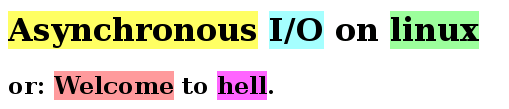
\includegraphics[width=.7\textwidth]{images/aio-linux.png}}\\
{\scriptsize (mirrored at \url{compgeom.com/~piyush/teach/4531_06/project/hell.html})}
   \\[2em]

   ``Asynchronous I/O, for example, is often infuriating.''\\
\hfill --- Robert Love. {\em Linux System Programming, 2nd ed, } page 215.

\end{center}

To motivate the need for non-blocking I/O, consider some standard I/O code:

\begin{lstlisting}[language=C]
    fd = open(...);
    read(...);
    close(fd);
\end{lstlisting}

This isn't very performant. The problem is that the {\tt read} call will
{\em block}. So, your program doesn't get to use the zillions of CPU cycles that
are happening while the I/O operation is occurring.

\paragraph{As seen previously: threads.} That can be fine if
you have some other code running to do work---for instance, other threads
do a good job mitigating the I/O latency, perhaps doing I/O themselves.
But maybe you would rather not use threads. Why not?

\begin{itemize}
\item potential race conditions;
\item overhead due to per-thread stacks; or
\item limitations due to maximum numbers of threads.
\end{itemize}

\paragraph{Non-blocking I/O.} The main point of this lecture, though,
is non-blocking/asynchronous I/O. The simplest example:

\begin{lstlisting}[language=C]
    fd = open(..., O_NONBLOCK);
    read(...); // returns instantly!
    close(fd);
\end{lstlisting}

In principle, the {\tt read} call is supposed to return instantly,
whether or not results are ready. That was easy!

Well, not so much. The {\tt O\_NONBLOCK} flag actually only has the
desired behaviour on sockets. The semantics of {\tt O\_NONBLOCK} is
for I/O calls to not block, in the sense that they should never wait
for data while there is no data available.

Unfortunately, files always have data available. Under Linux, you'd have
to use {\tt aio} calls to be able to send requests to the I/O subsystem
asynchronously and not, for instance, wait for the disk to spin up.
We won't talk about them, but they operate along the same lines as what
we will see. They just have a different API.

\paragraph{Conceptual view: non-blocking I/O.} Fundamentally,
there are two ways to find out whether I/O is ready to be queried:
polling (under UNIX, implemented via {\tt select}, {\tt poll},
and {\tt epoll}) and interrupts (under UNIX, signals).


We will describe {\tt epoll}. It is the most modern and
flexible interface. If you want to learn about \texttt{select} and \texttt{poll} at a lower level: \url{https://github.com/jzarnett/ece252/blob/master/lectures/L29-Asynchronous_I_O_with_select_poll.pdf }

The key idea is to give {\tt epoll} a bunch of file descriptors and
wait for events to happen. In particular:
     \begin{itemize}
       \item create an epoll instance ({\tt epoll\_create1});
       \item populate it with file descriptors ({\tt epoll\_ctl}); and
       \item wait for events ({\tt epoll\_wait}).
     \end{itemize}
Let's run through these steps in order.

\paragraph{Creating an {\tt epoll} instance.} Just use the API:
    \begin{lstlisting}[language=C]
   int epfd = epoll_create1(0);
    \end{lstlisting}

The return value {\tt epfd} is typed like a UNIX file
descriptor---{\tt int}---but doesn't represent any files; instead, use
it as an identifier, to talk to {\tt epoll}.

The parameter ``{\tt 0}'' represents the flags, but the only available flag
is {\tt EPOLL\_CLOEXEC}. Not interesting to you.

\paragraph{Populating the {\tt epoll} instance.} Next, you'll want
{\tt epfd} to do something. The obvious thing is to add some {\tt fd}
to the set of descriptors watched by {\tt epfd}:
    \begin{lstlisting}[language=C]
   struct epoll_event event;
   int ret;
   event.data.fd = fd;
   event.events = EPOLLIN | EPOLLOUT;
   ret = epoll_ctl(epfd, EPOLL_CTL_ADD, fd, &event);
    \end{lstlisting}

You can also use {\tt epoll\_ctl} to modify and delete descriptors from {\tt epfd}; read the manpage to find out how.

\paragraph{Waiting on an {\tt epoll} instance.} Having completed
the setup, we're ready to wait for events on any file descriptor in {\tt epfd}.
    \begin{lstlisting}[language=C]
  #define MAX_EVENTS 64

  struct epoll_event events[MAX_EVENTS];
  int nr_events;

  nr_events = epoll_wait(epfd, events, MAX_EVENTS, -1);
    \end{lstlisting}

The given {\tt -1} parameter means to wait potentially forever;
otherwise, the parameter indicates the number of milliseconds to wait.
(It is therefore ``easy'' to sleep for some number of milliseconds by
starting an {\tt epfd} and using {\tt epoll\_wait}; takes two function
calls instead of one, but allows sub-second latency.)

Upon return from {\tt epoll\_wait}, we know that we have {\tt
  nr\_events} events ready.

\subsection*{Level-Triggered and Edge-Triggered Events}
One relevant concept for these polling APIs is the concept of
\emph{level-triggered} versus \emph{edge-triggered}.  The default {\tt
  epoll} behaviour is level-triggered: it returns whenever data is
ready. One can also specify (via {\tt epoll\_ctl}) edge-triggered
behaviour: return whenever there is a change in readiness.

%\paragraph{Another Live Demo.} Now let's run some code (socket.c) that creates a
%server and reads from it, in either level-triggered mode or edge-triggered mode.

One would think that level-triggered mode would return from {\tt read}
whenever data was available, while edge-triggered mode would return
from {\tt read} whenever new data came in. Level-triggered does behave
as one would guess: if there is data available, {\tt read()} returns
the data. However, edge-triggered mode returns whenever the
state-of-readiness of the socket changes (from no-data-available to
data-available). Play with it and get a sense for how it works.

Good question to think about: when is it appropriate to choose one or the other?

\subsection*{Asynchronous I/O}
As mentioned above, the POSIX standard defines {\tt aio} calls.
Unlike just giving the {\tt O\_NONBLOCK} flag, using {\tt aio} works
for disk as well as sockets.

\paragraph{Key idea.} You specify the action to occur when I/O is ready:
    \begin{itemize}
      \item nothing;
      \item start a new thread; or
      \item raise a signal.
    \end{itemize}

Your code submits the requests using e.g. {\tt aio\_read} and {\tt aio\_write}.
If needed, wait for I/O to happen using {\tt aio\_suspend}.

\section*{Using cURL Asynchronously}
We've already seen that network communication is a great example of a way that you could use asynchronous  I/O. You can start a network request and move on to creating more without waiting for the results of the first one. For requests to different recipients, it certainly makes sense to do this.

The cURL multi interface has a lot of similarities with the regular cURL interface. Here's a simple example from \url{https://curl.haxx.se/libcurl/c/https.html} (i.e., the official docs):

\begin{lstlisting}[language=C]
#include <stdio.h>
#include <curl/curl.h>
 
int main( int argc, char** argv ) {
  CURL *curl;
  CURLcode res;
 
  curl_global_init(CURL_GLOBAL_DEFAULT);
 
  curl = curl_easy_init();
  if( curl ) {
    curl_easy_setopt(curl, CURLOPT_URL, "https://example.com/" );
    res = curl_easy_perform( curl );
    
  if( res != CURLE_OK ) {
      fprintf(stderr, "curl_easy_perform() failed: %s\n", curl_easy_strerror(res));
    }
    curl_easy_cleanup(curl);
  }
 
  curl_global_cleanup();
  return 0;
}
\end{lstlisting}

In the previous example, the call to \texttt{curl\_easy\_perform()} is blocking and we wait for the curl execution to take place. We want to change that! The tool for this is the ``multi handle'' - this is a structure that lets us have more than one curl easy handle. And rather than waiting, we can start them and then check on their progress. 

There are still the global initialization and cleanup functions. The structure for the new multi-handle type is \texttt{CURLM} (instead of \texttt{CURL}) and it is initialized with the \texttt{curl\_multi\_init()} function. 

Once we have a multi handle, we can add easy handles -- however many we need -- to the multi handle. Creation of the easy handle is the same as it is when being used alone - use \texttt{curl\_easy\_init()} to create it and then we can set however many options on this we need. Then, we add the easy handle to the multi handle with \texttt{curl\_multi\_add\_handle( CURLM* cm, CURL* eh )}.

Once we have finished putting all the easy handles into the multi handle, we can dispatch them all at once with \texttt{curl\_multi\_perform( CURLM* cm, int* still\_running )}. The second parameter is a pointer to an integer that is updated with the number of the easy handles in that multi handle that are still running. If it's down to 0, then we know that they are all done. If it's nonzero it means that some of them are still in progress.

This does mean that we're going to call\texttt{curl\_multi\_perform()} more than once. Doing so doesn't restart or interfere with anything that was already in progress -- it just gives us an update on the status of what's going on. We can check as often as we'd like, but the intention is of course to do something useful while the asynchronous I/O request(s) are going on. Otherwise, why not make it synchronous?

Suppose we've run out of things to do though. What then? Well, we can wait, if we want, using \texttt{curl\_multi\_wait( CURLM *multi\_handle, struct curl\_waitfd extra\_fds[], unsigned int extra\_nfds, int timeout\_ms, int *numfds )} . This function will block the current thread until something happens (some event occurs).

The first parameter is the multi handle, which makes sense. The second parameter is a structure of extra file descriptors you can wait on (but we will always want this to be NULL in this course) and the third parameter is the count (the size of the provided array) which would also be zero here. Then the second-last parameter is a maximum time to wait. The last parameter is a pointer that will be updated with the actual number of ``interesting'' events that occurred (interesting is the word used in the specifications, and what it means is mysterious). For a simple use case you can ignore most of the parameters and just wait for something to happen and go from there.

In the meantime though, the perform operations are happening, and so are whatever callbacks we have set up (if any). And as the I/O operation moves through its life cycle, the state of the easy handle is updated appropriately. Each easy handle has an associated status message as well as a return code.

Why both? Well - one is about what the status of the request is. The message could be, for example ``done'', but does that mean finished with success or finished with an error? For the second one tells us about that. We can ask about the status of the request using \texttt{curl\_multi\_info\_read( CURLM* cm, int* msgs\_left )}. This returns a pointer to information ``next'' easy handle, if there is one. The return value is a pointer to a struct of type \texttt{CURLMsg}. Along side this, the parameter \texttt{msgs\_left} is updated to say how many messages remain (so you don't have to remember or know in advance, really). 

We will therefore check the \texttt{CURLMsg} message to see what happened and make sure all is well. If our message that we got back with the info read is called \texttt{m}, What we are looking for is that the \texttt{m->msg} is equal to \texttt{CURLMSG\_DONE} -- request completed. If not, this request is still in progress and we aren't ready to evaluate whether it was successful or not. If there are more handles to look at, we should go on to the next. If it is done, we should look at the return code in and the result, in \texttt{m->data.result}. If it is \texttt{CURLE\_OK} then everything succeeded. If it's anything else, it indicates an error.

When a handle has finished, you need to remove it from the multi handle. A pointer to it is inside the \texttt{CURLMsg} under \texttt{m->easy\_handle}. It is removed with \texttt{curl\_multi\_remove\_handle( CURLM* cm, CURL eh )}. Once removed, it should be cleaned up like normal with \texttt{curl\_easy\_cleanup( CURL* eh )}.

There is of course the corresponding cleanup function \texttt{curl\_multi\_cleanup( CURLM * cm ) } for the multi handle when we are done with all the easy handles inside. The last step, as before, is to use the global cleanup function. After that we are done. 

Let's consider the following code example by Clemens Gruber~\cite{curlmulti}, with slight modifications for compactness, formatting, and to remember the cleanup. This example puts together all the things we talked about in one compact code segment. Here, the callback does nothing, but that's okay -- it's just to show what you could do with it.

\begin{lstlisting}[language=C]
#include <stdio.h>
#include <stdlib.h>
#include <unistd.h>
#include <curl/multi.h>

#define MAX_WAIT_MSECS 30*1000 /* Wait max. 30 seconds */

const char *urls[] = {
  "http://www.microsoft.com",
  "http://www.yahoo.com",
  "http://www.wikipedia.org",
  "http://slashdot.org"
};
#define CNT 4

size_t cb(char *d, size_t n, size_t l, void *p) {
  /* take care of the data here, ignored in this example */
  return n*l;
}

void init( CURLM *cm, int i ) {
  CURL *eh = curl_easy_init();
  curl_easy_setopt( eh, CURLOPT_WRITEFUNCTION, cb );
  curl_easy_setopt( eh, CURLOPT_HEADER, 0L );
  curl_easy_setopt( eh, CURLOPT_URL, urls[i] );
  curl_easy_setopt( eh, CURLOPT_PRIVATE, urls[i]) ;
  curl_easy_setopt( eh, CURLOPT_VERBOSE, 0L );
  curl_multi_add_handle( cm, eh );
}

int main( int argc, char** argv ) {
    CURLM *cm = NULL;
    CURL *eh = NULL;
    CURLMsg *msg = NULL;
    CURLcode return_code = 0;
    int still_running = 0; 
    int msgs_left = 0;
    int http_status_code;
    const char *szUrl;

    curl_global_init( CURL_GLOBAL_ALL );
    cm = curl_multi_init( );

    for ( int i = 0; i < CNT; ++i ) {
        init( cm, i );
    }

    curl_multi_perform( cm, &still_running );

    do {
        int numfds = 0;
        int res = curl_multi_wait( cm, NULL, 0, MAX_WAIT_MSECS, &numfds );
        if( res != CURLM_OK ) {
            fprintf( stderr, "error: curl_multi_wait() returned %d\n", res );
            return EXIT_FAILURE;
        }
        curl_multi_perform( cm, &still_running );

    } while( still_running );

    while ( ( msg = curl_multi_info_read( cm, &msgs_left ) ) ) {
        if ( msg->msg == CURLMSG_DONE ) {
            eh = msg->easy_handle;

            return_code = msg->data.result;
            if ( return_code != CURLE_OK ) {
                fprintf( stderr, "CURL error code: %d\n", msg->data.result );
                continue;
            }

            // Get HTTP status code
            http_status_code = 0;
            szUrl = NULL;

            curl_easy_getinfo( eh, CURLINFO_RESPONSE_CODE, &http_status_code );
            curl_easy_getinfo( eh, CURLINFO_PRIVATE, &szUrl );

            if( http_status_code == 200 ) {
                printf( "200 OK for %s\n", szUrl ) ;
            } else {
                fprintf( stderr, "GET of %s returned http status code %d\n", szUrl, http_status_code );
            }

            curl_multi_remove_handle( cm, eh );
            curl_easy_cleanup( eh );
        } else {
            fprintf( stderr, "error: after curl_multi_info_read(), CURLMsg=%d\n", msg->msg );
        }
    }
    curl_multi_cleanup( cm );
    curl_global_cleanup();
    return 0;
}
\end{lstlisting}

You may wonder about re-using an easy handle rather than removing and destroying it and making a new one. The official docs say that you can re-use one, but you have to remove it from the multi handle and then re-add it, presumably after having changed anything that you want to change about that handle. 

In this example all requests had the same (useless) callback, but of course you could have different callbacks for different easy handles if you wanted them to do different things. 


\section*{Building Servers: Concurrent Socket I/O}

\paragraph{Your Choices.} The first two both use blocking I/O, while the second two use
non-blocking I/O~~\cite{gplus:concurrent}:
    \begin{itemize}
      \item Blocking I/O; 1 process per request.
      \item Blocking I/O; 1 thread per request.
      \item Asynchronous I/O, pool of threads, callbacks, each thread handles multiple connections.
      \item Nonblocking I/O, pool of threads, multiplexed with select/poll,
        event-driven, each thread handles multiple connections.
    \end{itemize}

\paragraph{Blocking I/O; 1 process per request.}
This is the old Apache model.
  \begin{itemize}
    \item The main thread waits for connections.
    \item Upon connect, the main thread forks off a new process, which completely
      handles the connection.
    \item Each I/O request is blocking, e.g., reads wait until more data arrives.
  \end{itemize}

Advantage: 
  \begin{itemize}
    \item ``Simple to undertand and easy to program.''
  \end{itemize}

Disadvantage:
  \begin{itemize}
    \item High overhead from starting 1000s of processes.
      (We can somewhat mitigate this using process pools).
  \end{itemize}
This method can handle $\sim$10 000 processes, but doesn't generally scale beyond that, and
uses many more resources than the alternatives.

\paragraph{Blocking I/O; 1 thread per request.}
    We know that threads are more lightweight than processes. So let's use threads instead
of processes. Otherwise, this is the same as 1 process per request, but with less overhead.
I/O is the same---it is still blocking.

    Advantage:
    \begin{itemize}
      \item Still simple to understand and easy to program.
    \end{itemize}

    Disadvantages:
    \begin{itemize}
      \item Overhead still piles up, although less than processes.
      \item New complication: race conditions on shared data.
    \end{itemize}

\paragraph{Asynchronous I/O.} The other two choices don't assign one thread or process per connection,
but instead multiplex the threads to connections. We'll first talk
about using asynchronous I/O with select or poll.  

Here are (from 2006) some performance benefits of using asynchronous
I/O on lighttpd~\cite{lttpd}.

    \begin{tabular}{llrrr}
    version & & fetches/sec & bytes/sec & CPU idle \\
    1.4.13 & sendfile & 36.45 & 3.73e+06 & 16.43\% \\
    1.5.0 & sendfile & 40.51 & 4.14e+06 & 12.77\% \\
    1.5.0 & linux-aio-sendfile & 72.70 & 7.44e+06 & 46.11\% \\
    \end{tabular}

(Workload: $2\times 7200$ RPM in RAID1, 1GB RAM, transferring 10GBytes on a 100MBit network).

The basic workflow is as follows: 
   \begin{enumerate}
     \item enqueue a request;
     \item \ldots ~do something else;
     \item (if needed) periodically check whether request is done; and
     \item read the return value.
   \end{enumerate}

Some code which uses the Linux asynchronous I/O model is:
\begin{lstlisting}[language=C]
#include <aio.h>

int main() {
    // so far, just like normal
    int file = open("blah.txt", O_RDONLY, 0);

    // create buffer and control block
    char* buffer = new char[SIZE_TO_READ];
    aiocb cb;
    
    memset(&cb, 0, sizeof(aiocb));
    cb.aio_nbytes = SIZE_TO_READ;
    cb.aio_fildes = file;
    cb.aio_offset = 0;
    cb.aio_buf = buffer;

    // enqueue the read
    if (aio_read(&cb) == -1) { /* error handling */ }

    do {
      // ... do something else ...
    while (aio_error(&cb) == EINPROGRESS); // poll

    // inspect the return value
    int numBytes = aio_return(&cb);
    if (numBytes == -1) { /* error handling */ }

    // clean up
    delete[] buffer;
    close(file);
\end{lstlisting}

\paragraph{Using Select/Poll.} The idea is to improve performance
by letting each thread handle multiple connections.
When a thread is ready, it uses select/poll to find work:
    \begin{itemize}
      \item perhaps it needs to read from disk into a mmap'd tempfile;
      \item perhaps it needs to copy the tempfile to the network.
    \end{itemize}

In either case, the thread does work and updates the request state.

\bibliographystyle{alphaurl}
\bibliography{459}


\end{document}
